\begin{figure*}[htbp]
    \centering
    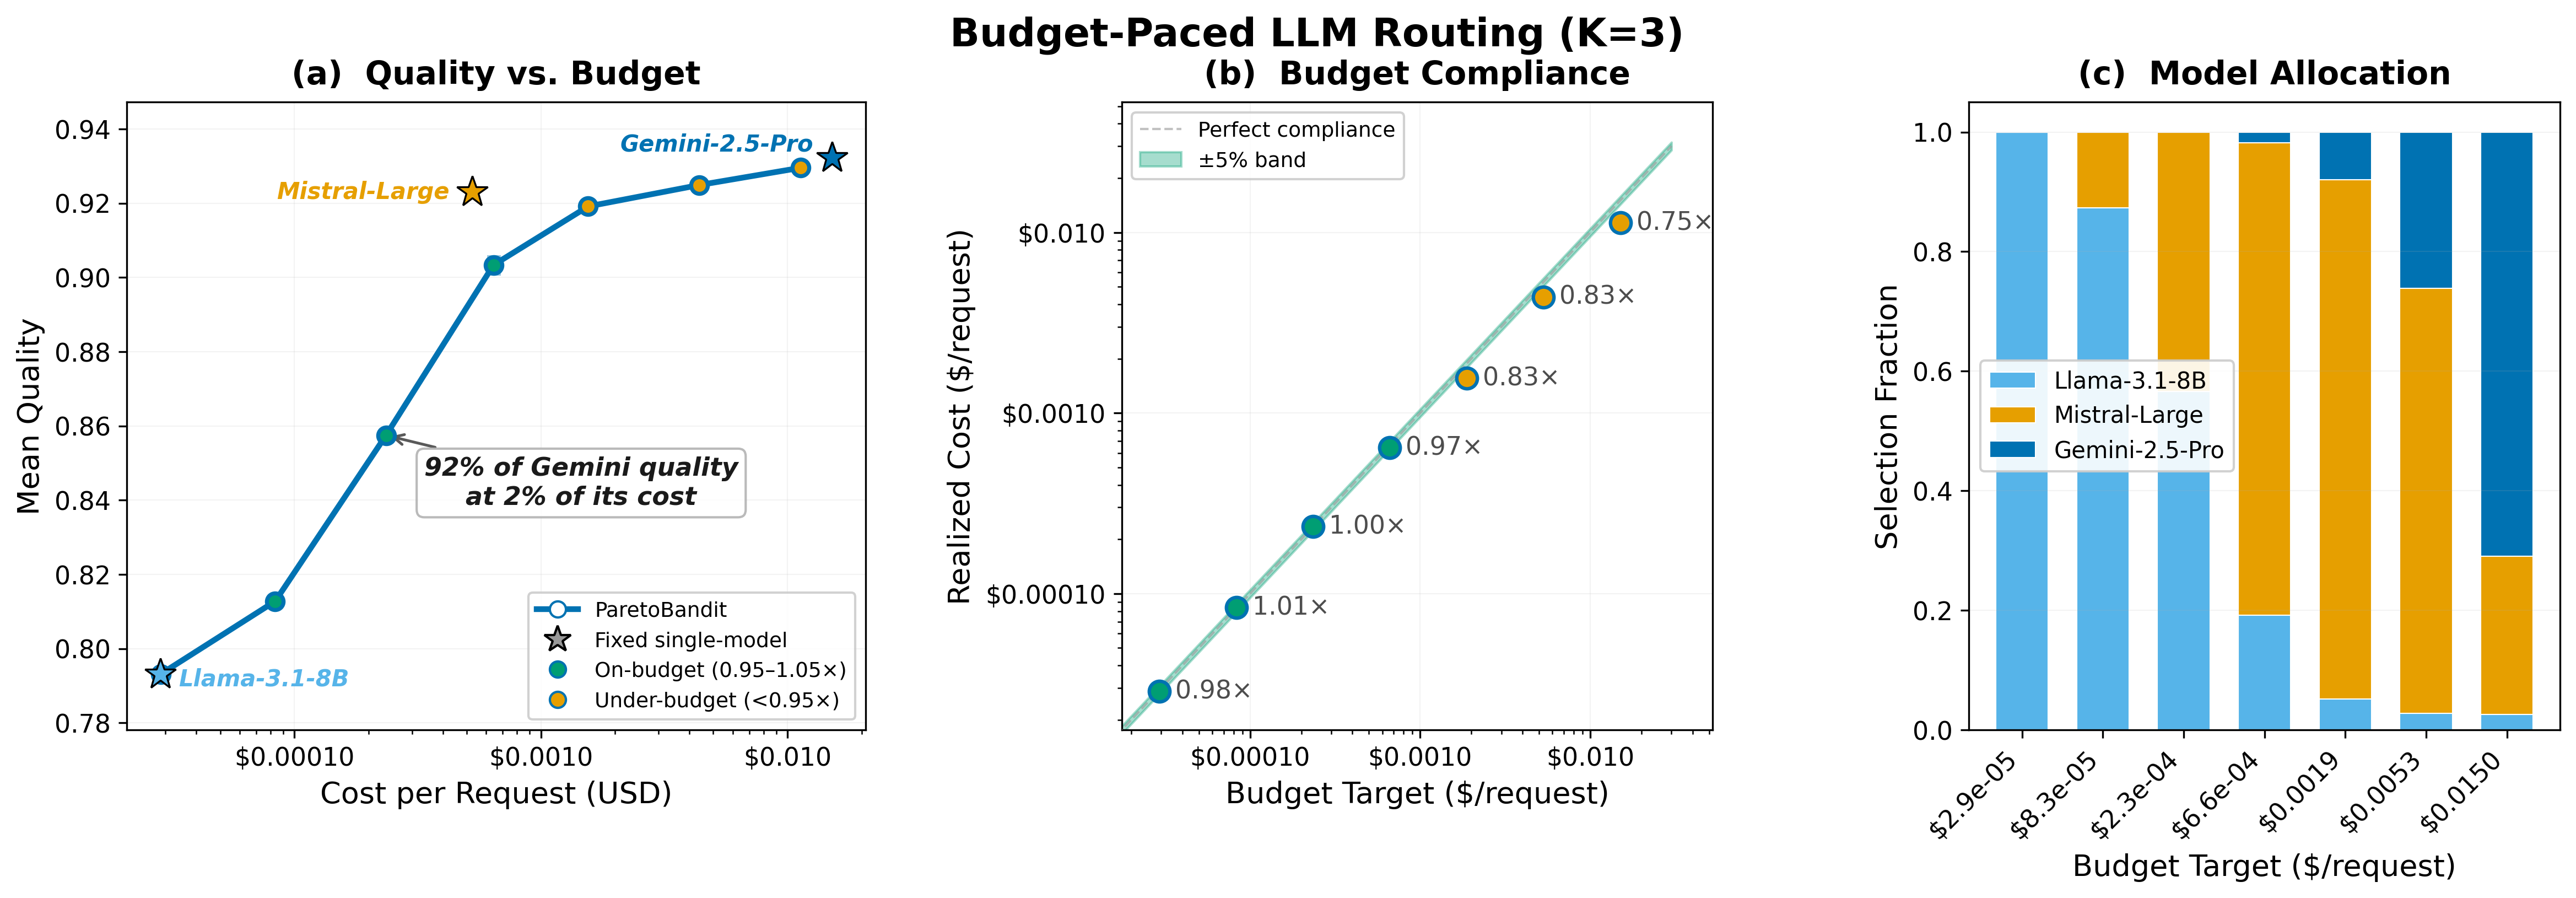
\includegraphics[width=\linewidth]{../experiments/01_stationary_budget_pacing/results/budget_pacing.pdf}
    \caption{Budget-paced LLM routing under stationary conditions
    ($K{=}3$: Llama-3.1-8B, Mistral-Large, Gemini-2.5-Pro;
    20~seeds, 95\% bootstrap CI).
    %
    \textbf{(a)~Quality vs.\ budget.}
    Each fixed model is a single operating point (star) at its
    inherent (cost, quality) coordinate.
    The ParetoBandit router (blue curve) traces a continuous
    quality--cost frontier by dynamically mixing models:
    it achieves \bpAnnotQualPct\% of Gemini-2.5-Pro quality at
    only \bpAnnotCostPct\% of its cost---an operating point
    no single model can reach.
    Marker fill indicates budget compliance:
    \textcolor[HTML]{009E73}{\textbf{green}} = on-target
    ($0.95$--$1.05\times$),
    \textcolor[HTML]{E69F00}{\textbf{orange}} = under-target
    ($< 0.95\times$).
    %
    \textbf{(b)~Budget compliance.}
    Realized cost vs.\ budget target; the dashed diagonal
    marks perfect compliance ($1.00\times$).
    For all binding targets the pacer achieves
    \bpUtilBindingLow--\bpUtilBindingHigh\ utilization.
    The loosest target under-spends (\bpLoosestUtil) because the
    router's unconstrained mean cost is already below that target.
    %
    \textbf{(c)~Model allocation.}
    At tight budgets the router routes nearly all traffic through
    Llama-3.1-8B; as budget increases, Mistral-Large enters the mix,
    and at loose budgets Gemini-2.5-Pro dominates---a smooth,
    principled transition driven by the dual variable $\lambda_t$.
    }
    \label{fig:budget_pacing}
\end{figure*}
